\documentclass[11pt,a4paper]{article}

\usepackage[T1]{fontenc}
\usepackage[utf8]{inputenc}
\usepackage[english]{babel}
\usepackage{lmodern}
\usepackage{amsmath}
\usepackage{booktabs}
\usepackage{graphicx}
\usepackage{caption}
\usepackage{siunitx}
\usepackage{hyperref}
\usepackage{geometry}
\geometry{margin=2.5cm}
\sisetup{detect-all}

\begin{document}

\begin{titlepage}
    \centering
    \vspace*{2cm}
    {\Large University Project Report\par}
    \vspace{1.5cm}
    {\huge\bfseries A Fortran Implementation of Conway's Game of Life\par}
    \vspace{0.7cm}
    {\Large with shared and distributed memory comparison\par}
    \vfill
    {\large Bastian Koberg\par}
    \vspace{0.5cm}
    {\large Advanced Scientific Programming\par}
    \vspace{0.5cm}
    {\large September 2026\par}
\end{titlepage}

\clearpage
\tableofcontents
\clearpage

\section{Introduction and problem formulation}

Conway's Game of Life is a simple rule-based simulation on a two-dimensional
grid. Each grid cell is either alive or dead. The state of the grid at step $t$
is
\begin{equation}
    u^t_{i,j} \in \{0,1\},
    \qquad i=1,\ldots,n_x,\quad j=1,\ldots,n_y .
\end{equation}
Here, $u^t_{i,j}=1$ denotes a living cell. To update one cell, the program
counts the eight cells directly around it. Their number is
\begin{equation}
    N^t_{i,j} =
    \sum_{a=-1\ne 0}^{1}\sum_{b=-1\ne 0}^{1}
    u^t_{i+a,j+b},
\end{equation}
 The update rule implemented by the program is
\begin{equation}
u^{t+1}_{i,j} =
\begin{cases}
1 \text{ if } u^t_{i,j}=1 \text{ and } N^t_{i,j}\in\{2,3\},\\
1 \text{ if } u^t_{i,j}=0 \text{ and } N^t_{i,j}=3,\\
0 \text{ otherwise.}
\end{cases}
\label{eq:gol-rule}
\end{equation}

In this implementation, the user can choose between periodic and dead walls as 
boundary conditions.choose wether to use periodic boundaries or dead walls. 
A random initial state is used for the benchmark runs, with about half of the 
cells alive at the start.

On first thought, one might expect this problem to be highly parallelizable,
because the update of each cell can be viewed as an independent pixel
operation. Once the state at time $t$ is known, every cell in the next grid
can be computed separately from the old grid. This makes the spatial part of
the problem well suited for parallel execution. The independence is not
complete, however: cells near a partition boundary require neighbour values
owned by another thread or MPI rank. These values must either be shared
through memory or exchanged explicitly as halo data, which introduces
communication and synchronization overhead. A further limitation is the time
dimension. Generation $t+1$ depends on the complete state of generation $t$,
so successive time steps cannot generally be computed in parallel. The
parallelism is therefore mainly within one generation, while the generations
themselves have to be processed sequentially. This explains why the update
kernel is suitable for parallelization, but the overall speedup is limited by
neighbour communication, synchronization, and the sequential progression in
time.

\section{Numerical and parallel implementation}

\subsection{Data flow and software architecture}
The project is written in Fortran and built with the Fortran Package
Manager (fpm). The main program in \texttt{app/main.f90} loads \texttt{params.json},
allocates two arrays, and advances the solution for the requested number of
frames. The numerical routines are in \texttt{src/gol\_utils.f90},
parameter parsing is isolated in \texttt{src/parameters.f90} and HDF5 output is handled
by \texttt{src/hdf5\_utils.f90}.

Two arrays are used: \texttt{board\_current} contains $u^t$ and
\texttt{board\_next} receives $u^{t+1}$. Every new cell reads only the old
state. For a grid with $n_x n_y$ cells and $F$ generations, the update work is
$\mathcal{O}(F n_x n_y)$ and the storage requirement is
$\mathcal{O}(n_x n_y)$ for the two boards.

The input used for the scaling data is $n_x=n_y=\texttt{base\_size}$,
$F=100$, periodic boundaries, and the random preset. The tested base sizes are
100, 500, 1000, 1250, and 1500. Every generated frame is written to an HDF5
dataset.

\subsection{Shared-memory implementation with OpenMP}
The nested loops for one generation use \texttt{omp do schedule(static)}. Rows
are distributed between threads. The input array is read-only during the loop,
and each iteration writes to a different element of \texttt{board\_next}.
Therefore, no critical section or reduction is needed. The two separate boards
also prevent a thread from reading cells that have already been changed in the
same step.

The neighbour routine handles the periodic boundaries and adds the eight
relevant cells. The parallel region is created for every generation. This is
simple, but thread management and memory access become important for small grids 
and higher generation counts.

\subsection{Distributed-memory implementation with MPI}
The MPI version uses a horizontal slab decomposition. Each MPI rank owns a
contiguous block of rows and stores two additional halo rows. Before every
generation, neighbouring ranks exchange their boundary rows using two
\texttt{MPI\_Sendrecv} operations. With periodic boundaries, the first and last
ranks communicate with each other as well.

The local update uses the same two-board scheme as the OpenMP version. When a
frame is saved, the local slabs are collected with \texttt{MPI\_Gatherv} on
rank 0, which writes the global frame to HDF5. This gives one common output
file, but halo exchange and the repeated gather add communication overhead.
OpenMP shares the arrays directly, while MPI must exchange boundary data
explicitly.


\section{Performance evaluation}

\subsection{Validation and runtime overview}
The Game of Life is deterministic so for a given initial grid and fixed boundary
conditions, every subsequent generation is uniquely determined. Consequently,
the same starting pattern must always produce the same sequence of patterns.
This property makes it possible to validate the implementation by comparing
its output with a known reference sequence. For this purpose, a fixed initial
pattern should be used instead of a newly generated random grid for every run.
For example, a small pattern consisting of vertical lines can be used as a
reproducible test case. Its evolution can be compared with an independent
cell-by-cell calculation using Eq.~\eqref{eq:gol-rule}.

The random initialisation used for the benchmarks does not provide the same
test: since the random distribution generates a different starting pattern in
each run, differences in the output cannot be attributed unambiguously to the
implementation. Therefore, validation should always use the identical fixed
initial pattern, while random initial states are appropriate for performance
measurements. The parallel versions should then be checked against the same
reference: one OpenMP thread and several OpenMP threads must produce identical
boards, and an MPI run with one rank must produce the same global frames as a
run with several ranks. This comparison also checks the halo indexing and slab
assembly. These deterministic pattern checks provide the validity check for
the performance measurements.

These checks confirmed that the OpenMP and MPI implementations produce the same
output as the serial version for the tested initial pattern. Although an error 
in the reference implementation cannot be ruled out completely, its behaviour 
is consistent with the specified update rules and it produces characteristic 
Game of Life patterns that are well established in the literature.\\

The first overview of the measured runtimes is given by the heatmaps in
Figs.~\ref{fig:openmp-heat} and~\ref{fig:mpi-heat}. The rows show the different
grid sizes and the columns show the number of threads or MPI ranks. Runtime
increases strongly with the grid size, while changing the number of processing
units produces only small improvements. The MPI heatmap also shows higher
runtimes again at eight ranks, which already indicates communication and output
overhead.

\begin{figure}[ht]
    \centering
    \begin{minipage}{0.48\textwidth}
        \centering
        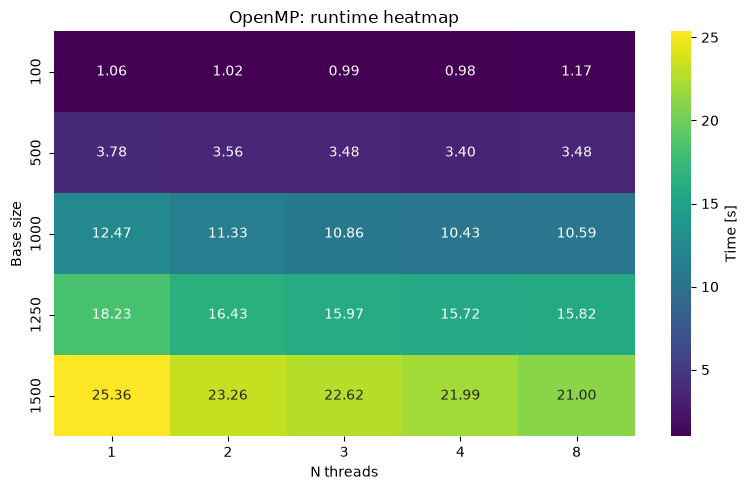
\includegraphics[width=\textwidth]{Pictures/openmp_heat.png}
        \captionof{figure}{OpenMP runtime for different grid sizes and thread counts.}
        \label{fig:openmp-heat}
    \end{minipage}\hfill
    \begin{minipage}{0.48\textwidth}
        \centering
        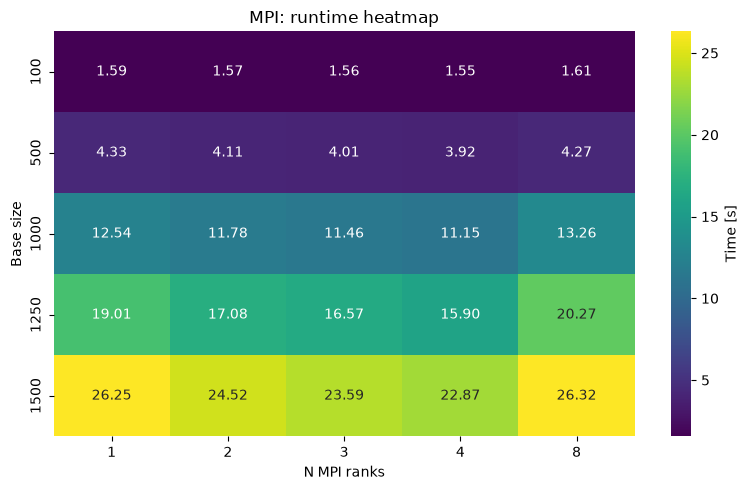
\includegraphics[width=\textwidth]{Pictures/mpi_heat.png}
        \captionof{figure}{MPI runtime for different grid sizes and rank counts.}
        \label{fig:mpi-heat}
    \end{minipage}
\end{figure}

\subsection{Strong scaling}
For strong scaling, the total grid size is kept fixed while the number of
threads or MPI ranks is changed. The speedup is
\begin{equation}
    S(P)=\frac{T_1}{T_P},
\end{equation}
where $T_P$ is the runtime with $P$ threads or MPI ranks.

The separate Strong-Scaling plots show runtime and speedup for OpenMP in
Fig.~\ref{fig:openmp-strong} and for MPI in Fig.~\ref{fig:mpi-strong}.
For both implementations, increasing the grid size increases the runtime much
more clearly than increasing the number of threads or ranks reduces it. The
nearly horizontal changes across processing elements show that the available
parallel speedup is small.



\begin{figure}[ht]
    \centering
    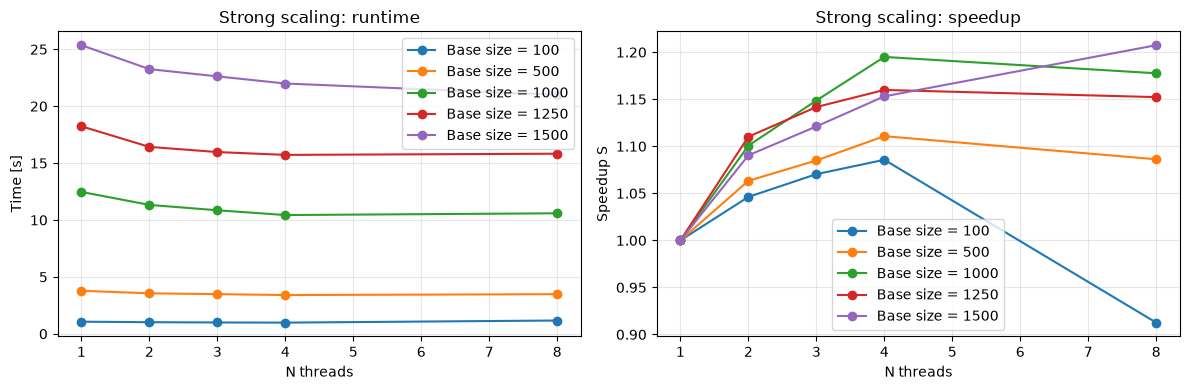
\includegraphics[width=0.98\textwidth]{Pictures/openmp_strong.png}
    \caption{OpenMP Strong Scaling: runtime and speedup for fixed grid sizes.}
    \label{fig:openmp-strong}
\end{figure}

\begin{figure}[ht]
    \centering
    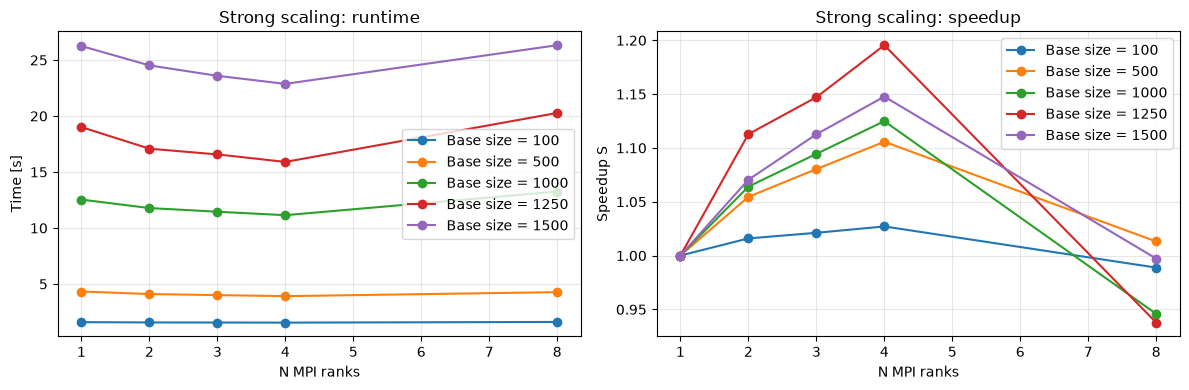
\includegraphics[width=0.98\textwidth]{Pictures/mpi_strong.png}
    \caption{MPI Strong Scaling: runtime and speedup for fixed grid sizes.}
    \label{fig:mpi-strong}
\end{figure}

The OpenMP speedup is best for the larger grids, but it remains far below ideal
linear scaling. For base size 1500, the runtime decreases from 25.36 seconds
with one thread to 21.00 seconds with eight threads, corresponding to a maximum
speedup of about 1.21. For base size 100, eight threads are slower than one.
The MPI curves show the same pattern: the best MPI speedup is about 1.20 at
four ranks for base size 1250, while eight ranks are slower again. Memory
access, thread management, communication, and HDF5 output all limit the
speedup.

The results show that OpenMP performs better than MPI for the tested workload.
Its shared-memory model avoids the explicit communication required by the
distributed-memory implementation, resulting in lower overhead and better
runtime behaviour. The MPI runtime increases again when the number of ranks is
raised to eight. At this point, halo exchange and the repeated collection of 
data for output outweigh the benefit of using additional ranks. The OpenMP 
runtime also shows limited improvement at higher thread counts, but its overhead
is lower and its performance remains more stable. Overall, the results indicate
that the update kernel itself is cheap, while memory access, communication, 
synchronization, and output dominate the total runtime and limit the achievable 
speedup.

\subsection{Weak scaling}
For weak scaling, the amount of work per thread or rank should stay constant
while the total problem size grows with $P$. The parallel efficiency is
\begin{equation}
    E(P)=\frac{S(P)}{P}=\frac{T_1}{P T_P},
\end{equation}
where the ideal value is $E(P)=1$.

The available runs keep the base size fixed instead of increasing it with $P$.
Therefore, the two Weak-Scaling plots should be read as runtime and efficiency
overviews of the available data, not as a strict weak-scaling experiment. The
OpenMP and MPI results are shown side by side in
Figs.~\ref{fig:openmp-weak} and~\ref{fig:mpi-weak}.
The heatmaps show that the runtime generally grows with the grid size, while
the changes along the processing-element axis are comparatively small. MPI
also shows a visible increase again at eight ranks for the larger grids, which
indicates that communication and output overhead become important.

\begin{figure}[ht]
    \centering
    \begin{minipage}{0.48\textwidth}
        \centering
        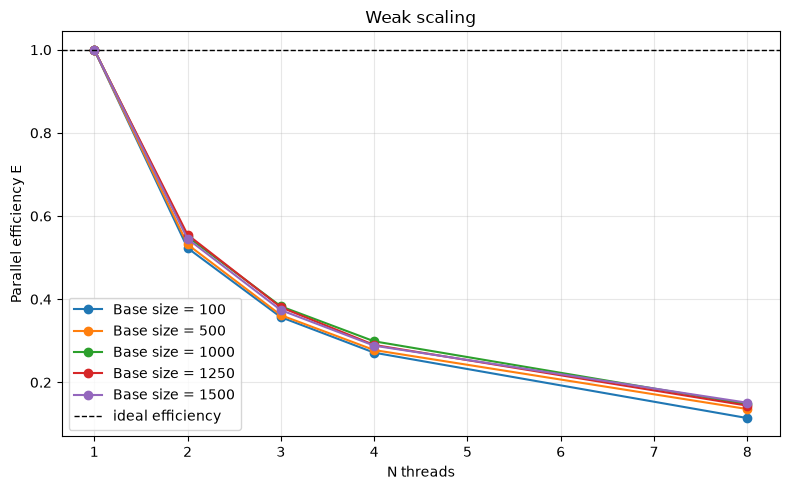
\includegraphics[width=\textwidth]{Pictures/openmp_weak.png}
        \captionof{figure}{OpenMP parallel efficiency for the available fixed-problem-size data.}
        \label{fig:openmp-weak}
    \end{minipage}\hfill
    \begin{minipage}{0.48\textwidth}
        \centering
        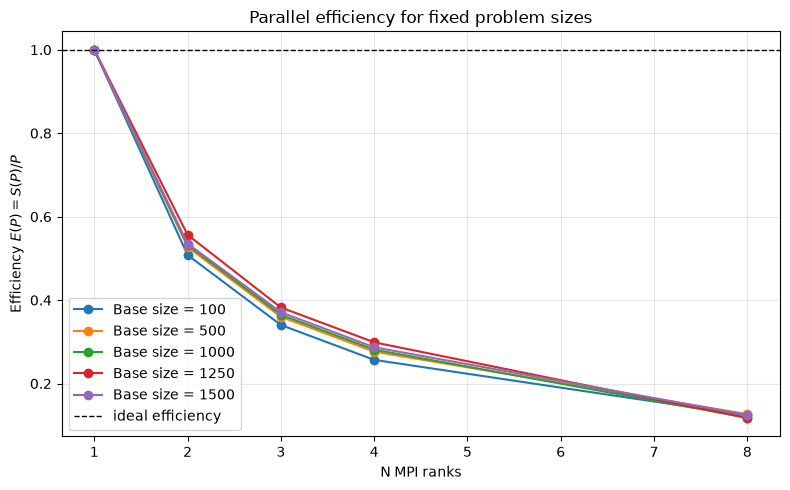
\includegraphics[width=\textwidth]{Pictures/mpi_weak.png}
        \captionof{figure}{MPI parallel efficiency for the available fixed-problem-size data.}
        \label{fig:mpi-weak}
    \end{minipage}
\end{figure}

The efficiency plots show a clear decrease as the number of threads or ranks
increases. For MPI, the curves for the different base sizes converge to nearly
the same low efficiency at eight ranks. This indicates that communication and
output overhead dominate the computation at higher rank counts, largely
independently of the problem size. The OpenMP results show a different trend:
at eight threads, the larger problem sizes retain a higher efficiency than the
smaller ones. The additional work of larger grids therefore amortizes the
thread-management and memory-access overhead more effectively. 

It would be interesting to investigate how the efficiency curves behave for
larger problem sizes and higher thread counts. The available data do not allow
a reliable conclusion, since the available hardware limited the experiments
to the tested number of CPU cores and threads. Nevertheless, the observed
trends suggest that the efficiency would fall well below 5 percent at higher
thread counts, as communication, memory access, and management overhead would
increasingly dominate the inexpensive update computation.

\subsection{MPI comparison and Amdahl's law}
Amdahl's model for strong scaling is
\begin{equation}
    S_A(P)=\frac{1}{(1-p)+p/P},
\end{equation}
where $p$ is the parallel fraction of the total runtime. Amdahl's law states
that only this fraction can benefit from additional threads or processes. From
the code, the cell-update loop is the main parallel part. In every generation,
however, it is accompanied by three full-array operations outside the parallel
region: resetting \texttt{board\_next}, copying \texttt{board\_next} to
\texttt{board\_current}, and resetting \texttt{board\_next} again. Approxmating 
the parallel fraction one can estimate a parallel fraction of $p \approx 0.20$ 
for the OpenMP version. The MPI version has additional communication and output 
overhead, so its parallel fraction is expected to be even lower.

The effective value measured for the complete application can be estimated
from a strong-scaling speedup using
\begin{equation}
    p=\frac{1-1/S(P)}{1-1/P}.
\end{equation}

\begin{table}[ht]
    \centering
    \caption{Effective parallel fraction estimated from the OpenMP speedups.}
    \label{tab:openmp-p}
    \begin{tabular}{c|rrrr}
        \toprule
        Base size & $p(P=2)$ & $p(P=3)$ & $p(P=4)$ & $p(P=8)$ \\
        \midrule
        100  & 0.088 & 0.099 & 0.105 & -0.109 \\
        500  & 0.119 & 0.117 & 0.133 &  0.091 \\
        1000 & 0.183 & 0.194 & 0.218 &  0.172 \\
        1250 & 0.198 & 0.186 & 0.184 &  0.151 \\
        1500 & 0.166 & 0.162 & 0.177 &  0.196 \\
        \bottomrule
    \end{tabular}
\end{table}

\begin{table}[ht]
    \centering
    \caption{Effective parallel fraction estimated from the MPI speedups.}
    \label{tab:mpi-p}
    \begin{tabular}{c|rrrr}
        \toprule
        Base size & $p(P=2)$ & $p(P=3)$ & $p(P=4)$ & $p(P=8)$ \\
        \midrule
        100  & 0.025 & 0.028 & 0.034 & -0.014 \\
        500  & 0.102 & 0.111 & 0.126 &  0.016 \\
        1000 & 0.121 & 0.129 & 0.148 & -0.066 \\
        1250 & 0.203 & 0.193 & 0.218 & -0.076 \\
        1500 & 0.132 & 0.152 & 0.172 & -0.003 \\
        \bottomrule
    \end{tabular}
\end{table}


The tables show that the effective parallel fraction increases with the problem
size. For the largest OpenMP problems, it approaches $p\approx0.2$; for
example, base size 1500 gives $p=0.196$ at eight threads. This agrees with the
approximated value and indicates that most of the
available speedup has already been obtained with eight threads. The smaller
grids have lower values because the fixed overhead is larger relative to the
actual update work.

The MPI results show a different behaviour at eight ranks. Several values of
$p$ become negative because the MPI runtime is higher than the serial runtime,
so the measured speedup is below one. A negative value does not mean that the
code contains a negative parallel fraction; it indicates that halo exchange,
synchronization, and frame collection introduce more overhead than the
parallel update can save. Overall, the measured values confirm that the
application reaches its strong-scaling limit early, with the largest useful
parallel fraction being only about 20 percent at 4 ranks.

\section{Conclusion}

This project studied a deterministic Game of Life implementation using both
OpenMP and MPI. The deterministic evolution allows the parallel versions to be
validated against a serial reference for the same initial pattern. The scaling
results show that the application is only poorly parallelizable for the tested
workload. Although the cell updates within one generation are independent, the
generations themselves must be processed sequentially, and each update is
relatively inexpensive compared with the memory operations, synchronization,
communication, and HDF5 output surrounding it.

OpenMP performs better on the shared-memory system and continues to benefit
from additional threads for the larger problem sizes, although the speedup
remains far below ideal. MPI reaches its best performance at approximately
four ranks; adding more ranks increases the communication and output overhead
and reduces the speedup again. 

More generally, these results illustrate that time-dependent problems are only
worthwhile to parallelize when each time step contains enough computation to
make up the associated overhead. Since the Game of Life update is very cheap,
the available parallelism is quickly outweighed by memory access and data
movement. 

\end{document}
